\chapter{Physics}

This chapter describes some of the physics and various conventions
\bmad uses. This chapter is by no means a comprehensive treatment
of accelerator physics and the interested reader is invited to consult 
any one of the number of good texts that deal with the subject\cite{b:wiedemann}.

%-----------------------------------------------------------------
\section{Units}
\label{s:units}
\index{units|hyperbf}

\index{MAD!units}
\index{units!with MAD}
\bmad uses SI (Syst\'eme International) units as shown in
Table~\ref{t:units}.  Note that \mad uses different units. For example,
\mad's unit of Particle Energy is GeV not eV.
\begin{table}[ht]
\centering
\begin{tabular}{|l|l|} \hline
  {\em Quantity}     & {\em Units}       \\ \hline
  Angles             &    radians        \\ 
  Betatron Phase     &    radians        \\
  Charge             &    Coulombs       \\
  Current            &    Amps           \\ 
  Frequency          &    Hz             \\ 
  Kick               &    radians        \\ 
  Length             &    meters         \\ 
  Magnetic Field     &    Tesla          \\ 
  Particle Energy    &    eV             \\ 
  Phase Angles (RF)  &    radians/2$\pi$ \\ 
  Voltage            &    Volts          \\ \hline
\end{tabular}
\caption{Physical units used by \bmad.}
\label{t:units}
\end{table}

%-----------------------------------------------------------------
\section{Magnetic Fields}
\label{s:fields}
\index{magnetic fields|hyperbf}

\index{MAD}
Start with the assumption that the local magnetic field has no
longitudinal component (obviously this assumption does not work with,
say, a solenoid).  Following \mad, the vertical magnetic field along
the $y = 0$ axis is expanded in a Taylor series
\Begineq
  B_y(x, 0) = \sum_n B_n \, \frac{x^n}{n!}
  \label{byx0b}
\Endeq
This is not the most
general form for the magnetic field. Essentially all of the skew
components have been ignored here. Assuming that the
reference orbit is locally straight (there are correction terms if the
Reference Orbit is locally curved), the field up to $3^{rd}$ order is
\begin{alignat}{5}
  B_x &=           &&B_1 y \plus         &&B_2 \, xy       
                   && \plus && \frac{1}{6} B_3 (3x^2 y - y^3) \plus \ldots \\
  B_y &= B_0 \plus &&B_1 x + \frac{1}{2} &&B_2 (x^2 - y^2) 
                   && \plus && \frac{1}{6} B_3 (x^3 - 3x y^2) \plus \ldots
\end{alignat}
The normalized integrated multipole $K_nL$ is used when specifying magnetic
multipole components
\index{multipole!KnL, Tn|hyperbf}
\Begineq
  K_nL \equiv \frac{q \, L \, B_n}{P_0}
\Endeq
$L \, B_n$ is the integrated multipole component over a length $L$,
and $P_0$ is the reference momentum. Note that $P_0/q$ is sometimes
written as $B\rho$. This is just an old notation where $\rho$ is the
bending radius of a particle with the reference energy in a field of
strength $B$. 

Conventionally, \bmad always takes the sign of the charge $q$ to be
positive. This means that, for example, positive $K_1$ and positive
$B_1$ are always associated with horizontally focusing quadrupoles for
positrons as well as electrons. The only element where the sign of the
particle's charge matters is an \vn{elseparator} element (\sref{s:elsep}).


The kicks $\Delta p_x$ and $\Delta p_y$ that a
particle experiences going through a multipole field is
\begin{alignat}{5}
  \Delta p_x & = \frac{-q \, L \, B_y}{P_0} \label{pqlbp1} \\
             & = -K_0 L \;-\; 
             && K_1 L \, x \plus 
             \frac{1}{2} && K_2 L (y^2 - x^2) && \plus 
             && \frac{1}{6} K_3 L (3x y^2 - x^3) \plus \ldots 
             \nonumber \\
  \Delta p_y & = \frac{q \, L \, B_x}{P_0} \label{pqlbp2} \\
             & =     
             && K_1 L \, y \plus 
             && K_2 L \, xy && \plus 
             && \frac{1}{6} K_3L (3x^2 y - y^3) \plus \ldots \nonumber 
\end{alignat}
A positive $K_1L$ quadrupole component gives
horizontal focusing and vertical defocussing. The general form is
\begin{align}
  \Delta p_x &= \sum_{n = 0}^{\infty} \frac{K_n L}{n!} 
             \sum_{m = 0}^{\lfloor \frac{n}{2} \rfloor}
             \begin{pmatrix} n \cr 2m \end{pmatrix} \,
             (-1)^{m+1} \, x^{n-2m} \, y^{2m} \\
  \Delta p_y &= \sum_{n = 0}^{\infty} \frac{K_n L}{n!} 
             \sum_{m = 0}^{\lfloor \frac{n-1}{2} \rfloor}
             \begin{pmatrix} n \cr 2m+1 \end{pmatrix} \,
             (-1)^{m} \, x^{n-2m-1} \, y^{2m+1}
\end{align}

\index{multipole!KnL, Tn|hyperbf}
So far only the normal components of the field have been
considered. If the fields associated with a particular $B_n$ multipole
component are rotated in the $(x, y)$ plane by an angle $\theta_n$, the
magnetic field at a point $(x,y)$ can be expressed in complex notation
as
\Begineq
  B_y(x,y) + i B_x(x,y) = 
    \frac{1}{n!} B_n e^{-i(n+1)\theta_n} \, e^{i n \theta} \, r^n 
  \label{bib1nb}
\Endeq
where $(r, \theta)$ are the polar coordinates of the point $(x, y)$.

\index{multipole!an, bn|hyperbf}
Another representation of the magnetic field used by \bmad divides
the fields into normal $b_n$ and skew $a_n$ components. In terms of
these components the magnetic field for the $n$\Th\ order multipole is
\Begineq
  \frac{q \, L}{P_0} \, (B_y + i B_x) = (b_n + i a_n) \, (x + i y)^n
\Endeq
The conversion between $(a_n, b_n)$ and $(K_nL, \theta_n)$ is
\Begineq
  b_n + i a_n = \frac{1}{n!} \, K_nL \, e^{-i(n+1)\theta_n}
\Endeq
or
\begin{align}
  K_n L &= n! \, \sqrt{a_n^2 + b_n^2} \\
  \tan[(n+1) \theta_n] &= \frac{-a_n}{b_n}
\end{align}
To convert a normal magnet (a magnet with no skew component) into a skew
magnet (a magnet with no normal component) the magnet should be rotated
about its longitudinal axis with a rotation angle of
\Begineq
  (n+1) \theta_n = \frac{\pi}{2}
\Endeq
For example, a normal quadrupole rotated by $45^\circ$ becomes a
skew quadrupole.

\index{ab_multipole}
\index{radius}
The $a_n$, $b_n$ representation of multipole fields is in
\vn{AB_Multipole} elements (\sref{s:ab.m}) as well as in other types
of elements such as quadrupoles, sextupoles, etc. This allows error
fields to be represented.  When $a_n$ and $b_n$ multipole values are
associated with an element that is not an \vn{AB_Multipole} element,
and if the \vn{scale_multipoles} attribute (\sref{s:multip}) is not
set to \vn{False}, a measurement radius $r_0$ and a scale factor $F$
are used to scale the effect of the $a_n$ and $b_n$ so that the
multipole strength scales as the element strength. The scaling formula
is
\Begineq
  \bigl[ a_n (\text{actual}), b_n (\text{actual}) \bigr] =
  \bigl[ a_n (\text{input}), b_n (\text{input}) \bigr] 
  \cdot F \cdot \frac{r_0^{n_\text{ref}}}{r_0^n} 
  \label{ababf}
\Endeq
$a_n(\text{input})$ and $b_n(\text{input})$ are the multipole values as given in the
lattice file. $a_n(\text{actual})$ and $b_n(\text{actual})$ are the multipole values
that are used in any simulation calculations. $r_0$ is set by the
\vn{radius} attribute of an element. $F$ and $n_\text{ref}$ are set
automatically depending upon the type of element as shown in
Table~\ref{t:ab}.

\index{ab_multipole}
\index{multipole}
Note that the $n = 0$ component of an \vn{AB_Multipole} or \vn{Multipole}
element rotates the reference orbit essentially acting as a zero length bend.
This is not true for multipoles that are associated with 
non-multipole elements.

\index{kicker}
\index{hkicker}
\index{vkicker}
\index{rbend}
\index{sbend}
\index{elseparator}
\index{quadrupole}
\index{solenoid}
\index{sol_quad}
\index{sextupole}
\index{octupole}
\begin{table}[ht]
\centering
\begin{tabular}{|l|l|l|} \hline
\tt
  {\em Element} & $F$                              & $n_\text{ref}$ \\ \hline
  \vn{Kicker}      & $\sqrt{{\tt Hkick}^2 + {\tt Vkick}^2}$ & 0 \\
  \vn{Hkicker}     & Kick                                   & 0 \\
  \vn{Vkicker}     & Kick                                   & 0 \\
  \vn{Rbend}       & G * L                                  & 0 \\
  \vn{Sbend}       & G * L                                  & 0 \\
  \vn{Elseparator} & $\sqrt{{\tt Hkick}^2 + {\tt Vkick}^2}$ & 0 \\
  \vn{Quadrupole}  & K1 * L                                 & 1 \\
  \vn{Solenoid}    & KS * L                                 & 1 \\
  \vn{Sol_Quad}    & K1 * L                                 & 1 \\
  \vn{Sextupole}   & K2 * L                                 & 2 \\
  \vn{Octupole}    & K3 * L                                 & 3 \\ \hline
\end{tabular}
\caption{$F$ and $n_\text{ref}$ for various elements.}
\label{t:ab}
\end{table}

%-----------------------------------------------------------------
\section{Taylor Maps and Symplectic Integration}
\label{s:taylor.phys}
\index{taylor map|hyperbf}
\index{symplectic integration}

A transport map ${\cal M}: {\cal R}^6 \rightarrow {\cal R}^6$ through
an element or a section of a lattice is a function that maps the
starting phase space coordinates $\Bf r(\In)$ to the ending
coordinates $\Bf r(\Out)$
\begin{equation}
  \Bf r(\Out) = {\cal M} \, \Bf r(\In)
\end{equation}
${\cal M}$ is made up of six functions ${\cal M}_i: {\cal R}^6
 \rightarrow {\cal R}$. Each of these functions maps to one of the $r(\Out)$
coordinates. These functions can be expanded in a Taylor
series and truncated at some order. Each Taylor series is in the form
\Begineq
  r_i(\Out) = \sum_{j = 1}^N \, C_{ij} \, \prod_{k = 1}^6 \, r_k^{e_{ijk}}(\In)
  \label{rcr}
\Endeq
Where the $C_{ij}$ are coefficients and the $e_{ijk}$ are integer exponents.
The order of the map is
\Begineq
  \mbox{order} = \max_{i,j} \left( \sum_{k = 1}^6 e_{ijk} \right)
\Endeq

The standard \bmad routine for printing a Taylor map might produce something 
like this: 
\begin{example}
   Taylor Terms:
    Out     Coef              Exponents           Order        Reference
   ---------------------------------------------------
      1:     -0.600000000000  0  0  0  0  0  0        0       0.200000000
      1:      1.000000000000  1  0  0  0  0  0        1
      1:      0.145000000000  2  0  0  0  0  0        2
   ---------------------------------------------------
      2:     -0.185000000000  0  0  0  0  0  0        0       0.000000000
      2:      1.300000000000  0  1  0  0  0  0        1
      2:      3.800000000000  2  0  0  0  0  1        3
   ---------------------------------------------------
      3:      1.000000000000  0  0  1  0  0  0        1       0.100000000
      3:      1.600000000000  0  0  0  1  0  0        1
      3:    -11.138187077310  1  0  1  0  0  0        2
   ---------------------------------------------------
      4:      1.000000000000  0  0  0  1  0  0        1       0.000000000
   ---------------------------------------------------
      5:      0.000000000000  0  0  0  0  0  0        0       0.000000000
      5:      0.000001480008  0  1  0  0  0  0        1
      5:      1.000000000000  0  0  0  0  1  0        1
      5:      0.000000000003  0  0  0  0  0  1        1
      5:      0.000000000003  2  0  0  0  0  0        2
   ---------------------------------------------------
      6:      1.000000000000  0  0  0  0  0  1        1       0.000000000
\end{example}
Each line in the example represents a single \vn{Taylor term}. The
Taylor terms are grouped into 6 \vn{Taylor series}. There is one
series for each of the output phase space coordinate. The first
column in the example, labeled ``out'', (corresponding to the $i$
index in \Eq{rcr}) indicates the Taylor series: $1 = x(out)$, $2 =
p_x(out)$, etc. The 6 exponent columns give the $e_{ijk}$ of
\Eq{rcr}. In this example, the second Taylor series (\vn{out} = 2),
when expressed as a formula, would read:
\Begineq
  p_x(out) = -0.185 + 1.3 \, p_x(in) + 3.8 \, x^2(in) \, p_z(in)
\Endeq

\index{taylor map!reference coordinates}
The reference column in the above example shows the input coordinates around
which the Taylor map is calculated. In this case, the reference
coordinates where 
\Begineq
  (x, p_x, y, p_y, z, p_z)_{ref} = (0.2, 0, 0.1, 0, 0, 0, 0)
\Endeq
The choice of the reference point will affect the values of the
coefficients of the Taylor map. For example, suppose that the exact
map through an element looks like
\Begineq
  x(out) = A \, \sin(k \, x(in))
\Endeq
Then a Taylor map to 1\St order is
\Begineq
  x(out) = c_0 + c_1 \, x(in)
\Endeq
where
\begin{align}
  c_1 &= A \, k \, \cos(k \, x_{\mbox{ref}}) \\
  c_0 &= A \, \sin(k \, x_{\mbox{ref}}) - c_1 \, x_{\mbox{ref}} \nonumber
\end{align}
Notice that once the coefficient values are determined the reference
point does not play any role when the Taylor map is evaluated to
determine the output coordinates as a function of the input
coordinates.

\index{taylor map!feed-down}
Of importance in working with Taylor maps is the concept of
\vn{feed-down}.  This is best explained with an example. To keep the
example simple, the discussion is limited to one phase space
dimension so that the Taylor maps are a single Taylor series. Take the
map $M_1$ from point 0 to point 1 to be
\Begineq
  M_1: x_1 = x_0 + 2
  \label{xx2}
\Endeq
and the map $M_2$ from point 1 to point 2 to be
\Begineq
  M_2: x_2 = x_1^2 + 3 \, x_1
  \label{xx3x}
\Endeq
Then concatenating the maps to form the map $M_3$ from point 0 to point 2
gives
\Begineq
  M_3: x_2 = (x_0 + 2)^2 + 3 (x_0 + 2) = x_0^2 + 7 \, x_0 + 10
  \label{xx23x2}
\Endeq
However if we are evaluating our maps to only 1\St order the map $M_2$
becomes
\Begineq
  M_2: x_2 = 3 \, x_1
\Endeq
and concatenating the maps now gives
\Begineq
  M_3: x_2 = 3 (x_0 + 2) = 3 \, x_0 + 6
  \label{x3x23}
\Endeq
Comparing this to \Eq{xx23x2} shows that by neglecting the 2\Nd order
term in \Eq{xx3x} leads to 0\Th and 1\St order errors in
\Eq{x3x23}. These errors can be traced to the finite 0\Th order term in
\Eq{xx2}. This is the principal of feed--down: Given $M_3$ which is a map
produced from the concatenation of two other maps, $M_1$, and $M_2$
\Begineq
  M_3 = M_2(M_1)
\Endeq
Then if $M_1$ and $M_2$ are correct to n\Th order, $M_3$ will also be
correct to n\Th order as long as $M_1$ has no constant (0\Th order)
term. [Notice that a constant term in $M_2$ does not affect the
argument.]  What happens if we know there are constant terms in our
maps? One possibility is to go to a coordinate system where the
constant terms vanish. In the above example that would mean using the
coordinate $\widetilde x_0$ at point 0 given by
\Begineq
  \widetilde x_0 = x_0 + 2
\Endeq
\index{symplectic integration}
The other possibility is to use symplectic integration. By its nature,
symplectic integration never has problems with feed--down.

The subject of symplectic integration is too large to be covered in
this guide. The reader is referred to the book ``Beam Dynamics: A New
Attitude and Framework'' by Etienne Forest\cite{b:forest}. A brief
synopsis: Symplectic integration uses as input 1) The Hamiltonian that
defines the equations of motion, and 2) a Taylor map $M_1$ from point 0 to
point 1. Symplectic integration from point 1 to point 2 produces a
Taylor map $M_3$ from point 0 to point 2. Symplectic integration can
produce maps to arbitrary order. In any practical application the
order $n$ of the final map is specified and in the integration
procedure all terms of order higher than $n$ are ignored. If one is
just interested in knowing the final coordinates of a particle at
point 2 given the initial coordinates at point 1 then $M_1$ is just
the constant map
\Begineq
  M_1: x_1 = c_i
\Endeq
where $c_i$ is the initial starting point. The order of the
integration is set to 0 so that all non--constant terms are
ignored. The final map is also just a constant map
\Begineq
  M_3: x_2 = c_f
\Endeq
If the map from point 1 to point 2 is desired then the map $M_1$ is
just set to the identity map
\Begineq
  M_1: x_1 = x_0
\Endeq
In general it is impossible to exactly integrate any non--linear
system. In practice, the symplectic integration is achieved by slicing
the interval between point 1 and point 2 into a number of (generally
equally spaced) slices. The integration is performed, slice step by
slice step. This is analogous to integrating a function by evaluating
the function at a number of points. Using more slices gives better
results but slows down the calculation. The speed and accuracy of the
calculation is determined by the number of slices and the \vn{order}
of the integrator. The concept of integrator order can best be
understood by analogy by considering the trapezoidal rule for
integrating a function of one variable:
\Begineq
  \int_{y_a}^{y_b} f(y) \, dy = 
  h \left[ \frac{1}{2} f(y_a) + \frac{1}{2} f(y_b) \right] +
  o(h^3 \, f^{(2)})
\Endeq
In the formula $h = y_b - y_a$ is the slice width. $0(h^3 \, f^{(2)})$
means that the error of the trapezoidal rule scales as the second
derivative of $f$. Since the error scales as $f^{(2)}$ this is an
example of a second order integrator. To integrate a function between
points $y_1$ and $y_N$ we slice the interval at points $y_2 \ldots y_{N-1}$
and apply the trapezoidal rule to each interval. Examples of higher
order integrators can be found, for example, in Numerical
Recipes\cite{b:nr}. The concept of integrator order in symplectic
integration is analogous. 

The optimum number of slices is determined by the smallest number that
gives an acceptable error. The slice size is given by the \vn{ds_step}
attribute of an element (\sref{s:integ}).  Integrators of higher order
will generally need a smaller number of slices to achieve a given
accuracy. However, since integrators of higher order take more time
per slice step, and since it is computation time and not number of
slices which is important, only a measurement of error and calculation
time as a function of slice number and integrator order will
unambiguously give the optimum integrator order and slice width.  In
doing a timing test, it must be remembered that since the magnitude of
any non-linearities will depend upon the starting position, the
integration error will be dependent upon the starting map $M_1$. \bmad
has integrators of order 2, 4, and 6 (\sref{s:integ}). Timing tests
performed for some wiggler elements (which have strong nonlinearities)
showed that, in this case, the 2\Nd order integrator gave the fastest
computation time for a given accuracy. However, the higher order
integrators may give better results for elements with weaker
nonlinearities.

%-----------------------------------------------------------------
\section{Symplectification}
\label{s:symp.method}
\index{symplectification}

If the evolution of a system can be described using a Hamiltonian then
it can be shown that the linear part of any transport map (the Jacobian)
must obey the symplectic condition. If a matrix $\Bf M$ is not symplectic,
Healy\cite{b:healy} has provided an elegant method for finding a symplectic 
matrix that is ``close'' to $\Bf M$. The procedure is as follows:
From $\Bf M$ a matrix $\bV$ is formed via
\begin{equation}
  \bV = \Bf S (\Bf I - \Bf M)(\Bf I + \Bf M)^{-1} 
  \label{e:vsimi}
\end{equation}
where $\Bf S$ is the matrix
\Begineq
  \Bf S = 
  \begin{pmatrix} 
      0 &  1 &  0 &  0 &  0 &  0 \cr
     -1 &  0 &  0 &  0 &  0 &  0 \cr
      0 &  0 &  0 &  1 &  0 &  0 \cr
      0 &  0 & -1 &  0 &  0 &  0 \cr
      0 &  0 &  0 &  0 &  0 & -1 \cr
      0 &  0 &  0 &  0 & -1 &  0 \cr
  \end{pmatrix}
  \label{s0100}
\Endeq
$\bV$ is symmetric if and only if $\Bf M$ is symplectic. In any case,
a symmetric matrix $\Bf W$ near $\bV$ can be
formed via
\begin{equation}
  \Bf W = \frac{\bV + \bV^t}{2}
\end{equation}
A symplectic matrix $\Bf F$ is now obtained by inverting \eq{e:vsimi}
\Begineq
  \Bf F = (\Bf I + \Bf S \Bf W) (\Bf I - \Bf S \Bf W)^{-1}
\Endeq

%-----------------------------------------------------------------
\section{LINAC Accelerating Cavities (Lcavity)}
\label{s:lcav.phys}

The transverse trajectory through an \vn{Lcavity} is modeled using equations
developed by Rosenzweig and Serafini\cite{b:rosenzweig} with
\Begineqs
  b_0 &= 1 \CRNO
  b_{-1} &= 1 
\Endeqs
and all other $b_n$ set to zero.

The transport through the body (R\&S Eq.~(9)) has been modified to give the 
correct phase-space area at non ultra-relativistic energies:
\Begineq
  \begin{pmatrix}
    x \\ 
    x'
  \end{pmatrix}_2 = 
  \begin{pmatrix}
    m_{11}                      & \beta_1 \, m_{12} \\
    \frac{1}{\beta_2} \, m_{21} & \frac{\beta_1}{\beta_2} \, m_{22} 
  \end{pmatrix}
  \,
  \begin{pmatrix}
    x \\ 
    x'
  \end{pmatrix}_1
\Endeq
where the $m_{ij}$ are the matrix elements from R\&S Eq.~(9) and the 
$\beta$ are the standard relativistic factors. With this, the determinate 
of the matrix is $\beta_1 \, \gamma_1 / \beta_2 \, \gamma_2$.

The change in $z$ going through a cavity is calculated by first calculating the particle
transit time $\Delta t$
\begin{align}
  c \, \Delta t &= \int_{s_1}^{s_2} \!\! ds \,\, \frac{1}{\beta(s)} \CRNO
  &= \int_{s_1}^{s_2} \!\! ds \, \frac{E}{\sqrt{E^2 - (mc^2)^2}} \\
  &= \frac{c \, P_{z2} - c \, P_{z1}}{G} \nonumber
\end{align}
where it has been assumed that the accelerating gradient $G$ is
constant through the cavity. In this equation $\beta = v / c$, $E$ is
the energy, and $P_{z1}$ and $P_{z2}$ are the entrance and exit
momenta. Using \Eq{zbctt}, the change in $z$ is thus
\Begineq
  z_2 = \frac{\beta_2}{\beta_1} \, z_1 - 
  \beta_2 \, 
  \left(
  \frac{c \, P_{z2} - c \, P_{z1}}{G} - 
  \frac{c \, \BAR P_{z2} - c \, \BAR P_{z1}}{\BAR G}
  \right)
\Endeq
where $\BAR P$ and $\BAR G$ are the momentum and gradient of the
reference particle.

%-----------------------------------------------------------------
\section{Synchrotron Radiation Damping and Excitation}
\label{s:radiation}
\index{synchrotron radiation!damping and excitation|hyperbf}

Emission of synchrotron radiation by a particle can be decomposed into
two parts. The deterministic average radiation emitted produces damping
while the stochastic fluctuating part produces excitation\cite{b:jowett}.

\index{MAD!radiation}
The treatment of radiation damping by \bmad essentially follows \mad.
The average change in energy $\Delta E$ of a particle going through a
section of magnet due to synchrotron radiation is
\Begineq
  \frac{\Delta E}{E_0} = -k_d \, (1 + p_z)
\Endeq
where
\Begineq
  k_d \equiv \frac{2 \, r_e}{3} \, \gamma_0^3 \, \ave{g_0^2} \, L_p \,  
  (1 + p_z)
  \label{k2r3g}
\Endeq
$r_e$ is the classical electron radius, $L_p$ is the actual path
length, $\gamma_0$ is the energy factor of an on-energy particle, $1/g_0$
is the bending radius of an on--energy particle, and $\ave{g_0^2}$ is an
average of $g_0^2$ over the actual path.

The energy lost is given by
\Begineq
  \frac{\Delta E}{E_0} = -k_f \, (1 + p_z)
\Endeq
where
\Begineq
  k_f \equiv \left( \frac{55 \, r_e \, \hbar \, c}{24 \, \sqrt{3} \, m_e} \, 
  L_p \, \gamma_0^5 \ave{g_0^3} \right)^{1/2} \, (1 + p_z) \, \xi
  \label{k55rh}
\Endeq
$\xi$ is a Gaussian distributed random number with unit sigma and zero mean.

Using \Eqs{k2r3g} and \eq{k55rh} the total change in $p_z$ can be written as
\Begineq
  \Delta p_z = \frac{\Delta E}{E_0} = -k_E \, (1 + p_z)
\Endeq
where
\Begineq
  k_E = k_d + k_f
\Endeq
Since the radiation is emitted in the forward direction the angles
$x'$ and $y'$ are invariant which leads to the following equations for
the changes in $p_x$ and $p_y$
\begin{align}
  \Delta p_x &= -k_E \, p_x \CRNO
  \Delta p_y &= -k_E \, p_y 
\end{align}

The above formalism does not take into account the fact that radiation is 
emitted with a $1/\gamma$ angular distribution. This means that the calculated
vertical emittance for a lattice with
bends only in the horizontal plane and without any coupling elements such as
skew quadrupoles will be zero. Typically, in practice, the vertical emittance
will be dominated by coupling so this approximation is generally a good one.

%-----------------------------------------------------------------
\section{Coupling and Normal Modes}
\label{s:coupling}
\index{normal mode!Coupling}

The coupling formalism used by \bmad is taken from the paper of Sagan
and Rubin\cite{b:coupling}. The main equations are reproduced here.  A
one--turn map $\bfT(s)$ for the transverse two--dimensional phase space
$\bfx = (x, x', y, y')$ starting and ending at some point $s$ can be
written as
  \Begineq
    \bfT = \bfV \, \bfU \, \bfV\inv 
    , \label{tvuv}
  \Endeq 
where $\bfV$ is symplectic, and $\bfU$ is of the form
  \Begineq
    \bfU = 
    \begin{pmatrix}
      \bfA & \Bf0 \cr 
      \Bf0 & \bfB \cr
    \end{pmatrix}
    . \label{ua00b}
  \Endeq
\index{normal mode!a--mode}
\index{normal mode!b--mode}
Since $\bfU$ is uncoupled the standard Twiss analysis can be
performed on the matrices $\bfA$ and $\bfB$. The normal modes
are labeled $a$ and $b$ and if the one--turn matrix $\bfT$ is
uncoupled then $a$ corresponds to the horizontal mode and $b$
corresponds to the vertical mode. 

$\bfV$ is written in the form
  \Begineq
    \bfV = 
    \begin{pmatrix}
        \gamma \bfI & \bfC \cr 
        -\bfC^+     & \gamma \bfI \cr
    \end{pmatrix}
    , \label{vgicc1}
  \Endeq
where $\bfC$ is a 2x2 matrix and $+$ superscript 
denotes the symplectic conjugate:
\index{symplectic!conjugate}
  \Begineq
    \bfC^+ = 
    \begin{pmatrix}
       C_{22} & -C_{12} \cr 
      -C_{21} & C_{11} \cr
    \end{pmatrix}
    . \label{ccccc}
  \Endeq
Since we demand that $\bfV$ be symplectic we have the condition
  \Begineq               
    \gamma^2 + \, ||\bfC|| = 1
    , \label{gc1}
  \Endeq
and $\bfV\inv$ is given by
  \Begineq
    \bfV\inv = 
    \begin{pmatrix}
      \gamma \bfI & -\bfC \cr 
      \bfC^+ & \gamma \bfI \cr
    \end{pmatrix}
    . \label{vgicc2}
  \Endeq 
$\bfC$ is a measure of the coupling. 
$\bfT$ is uncoupled if and only if $\bfC = \Bf 0$. 

It is useful to normalize out the $\beta(s)$ variation in the the above
analysis. Normalized quantities being denoted by a bar above them. The
normalized normal mode matrix $\BAR\bfU$ is defined by
  \Begineq
    \BAR\bfU = \bfG \, \bfU \, \bfG\inv
    , \label{ugug}
  \Endeq
Where $\bfG$ is given by 
  \Begineq
    \bfG \equiv 
    \begin{pmatrix}
      \bfG_a & \Bf0 \cr 
      \Bf0 & \bfG_b
    \end{pmatrix}
    , \label{gg00g}
  \Endeq  
with 
  \Begineq
    \bfG_a = 
    \begin{pmatrix}
      \frac{\tstyle 1}{\tstyle \sqrt{\beta_a}} & 0 \cr
      \frac{\tstyle \alpha_a}{\tstyle \sqrt{\beta_a}} & \sqrt{\beta_a}
    \end{pmatrix}
    , \label{g1b0a} 
  \Endeq
with a similar equation for $\bfG_b$. With this definition, the corresponding
$\BAR\bfA$ and $\BAR\bfB$ (cf.~\Eq{ua00b}) are just rotation matrices.
The relationship between $\bfT$ and $\BAR\bfU$ is 
  \Begineq
    \bfT = \bfG\inv \, \BAR\bfV \, \BAR\bfU \, \BAR\bfV\inv \, \bfG
    , \label{tgvuv}
  \Endeq
where
  \Begineq
    \BAR\bfV = \bfG \, \bfV \, \bfG\inv
    . \label{vgvg}
  \Endeq
Using \Eq{gg00g}, $\BAR\bfV$ can be written in the form
  \Begineq
    \BAR\bfV = 
    \begin{pmatrix}
      \gamma \bfI & \BAR\bfC \cr -\BAR\bfC^+ & \gamma \bfI
    \end{pmatrix}
    , \label{vgicc3}
  \Endeq
with the normalized matrix $\BAR\bfC$ given by
  \Begineq
    \BAR\bfC = \bfG_a \, \bfC \, \bfG_b\inv
    . \label{cgcg}
  \Endeq

The normal mode coordinates ${\bf a} = (a, a', b, b')$ are related to
the laboratory frame via
  \Begineq
    {\bf a} = \bfV\inv \, {\bf x}
    . \label{avx}
  \Endeq 
In particular the normal mode dispersion $\bfeta_a = (\eta_a,
\eta'_a, \eta_b, \eta'_b)$ is related to the laboratory frame
dispersion $\bfeta_x = (\eta_x, \eta'_x, \eta_y, \eta'_y)$ via
  \Begineq
    {\bfeta_a} = \bfV\inv \, {\bfeta_x}
    . \label{etaavx}
  \Endeq 
When there is no coupling ($\bfC = 0$), $\bfeta_a$ and $\bfeta_x$ are
equal to each other.

%-----------------------------------------------------------------
\section{Dispersion Calculation}
\label{s:dispersion}
\index{dispersion|hyperbf}

The dispersion ($\eta$) and the dispersion derivative ($\eta'$) are 
defined by the equations
\begin{align}
  \eta_x(s) &\equiv \left. \frac{dx}{dp_z} \right|_s \comma \qquad
    \eta'_x(s) \equiv \left. \frac{d\eta_x}{ds} \right|_s
    = \left. \frac{dx'}{dp_z} \right|_s \CRNO
  \eta_y(s) &\equiv \left. \frac{dy}{dp_z} \right|_s \comma \qquad
    \eta'_y(s) \equiv \left. \frac{d\eta_y}{ds} \right|_s
    = \left. \frac{dy'}{dp_z} \right|_s \\
  \eta_z(s) &\equiv \left. \frac{dz}{dp_z} \right|_s \nonumber
\end{align}

Given the dispersion at a given point, the dispersion at some other
point is calculated as follows: Let $\Bf r = (x, p_x, y, p_y, z, p_z)$
be the reference orbit, around which the dispersion is to be
calculated. Let $\bV$ and $\bf M$ be the zeroth and first order components of 
the transfer map between two points labeled 1 and 2:
\Begineq
  \Bf r_2 = \bM \, \Bf r_1 + \bV
  \label{rmrv}
\Endeq
Define the dispersion vector $\bfeta$ by
\Begineq
  \bfeta = 
  \left( 
    \eta_x, \eta'_x \, (1 + p_z), \eta_y, \eta'_y \, (1 + p_z), \eta_z, 1
  \right)
\Endeq
Differentiating \Eq{rmrv} with respect to energy, 
the dispersion at point 2 in terms of the dispersion at point 1 is
\Begineq
  \bfeta_2 = \frac{dp_{z1}}{dp_{z2}} \left[ \bM \, \bfeta_1 \right] + \bV_\eta 
\Endeq
where
\Begineq
  \bV_\eta = \frac{dp_{z1}}{dp_{z2}} \, \frac{1}{1 + p_{z1}}
  \left(
  \begin{array}{c}
    M_{12} \, p_{x1} + M_{14} \, p_{y1} \\
    M_{22} \, p_{x1} + M_{24} \, p_{y1} \\
    M_{32} \, p_{x1} + M_{34} \, p_{y1} \\
    M_{42} \, p_{x1} + M_{44} \, p_{y1} \\
    M_{52} \, p_{x1} + M_{54} \, p_{y1} \\
    M_{62} \, p_{x1} + M_{64} \, p_{y1} \\
  \end{array}
  \right)
  -
  \left(
  \begin{array}{c}
    0 \\
    \frac{p_{x2}}{1 + p_{z2}} \\
    0 \\
    \frac{p_{y2}}{1 + p_{z2}} \\
    0 \\
    0 
  \end{array}
  \right)
\Endeq
The sixth row of the matrix equation gives $dp_{z1}/dp_{z2}$. 
Explicitly
\Begineq
  \left[ \frac{dp_{z1}}{dp_{z2}} \right]^{-1} =
  \sum_{i=1}^6 M_{6i} \, \eta_{1i} + 
  \frac{M_{62} \, p_{x1} + M_{64} \, p_{y1}}{1 + p_{z1}}
\Endeq
For everything except \vn{RFcavity} and \vn{Lcavity} elements, 
$dp_{z1}/dp_{z2}$ is 1.

%-----------------------------------------------------------------
\section{Instrumental Measurements}
\label{s:meas.calc}
\index{measurement}

\bmad has the ability to simulate instrumental measurement errors
for orbit, dispersion, betatron phase, and coupling measurements.
The appropriate attributes are listed in \sref{s:meas.attrib} and
the conversion formulas are outlined below.

%-----------------------------------------------------------------
\subsection{Orbit Measurement}
\index{orbit!measurement}

For orbits, the
relationship between measured position $(x, y)_{\mss{meas}}$ and true position 
$(x, y)_{true}$ is
\Begineq
  \begin{pmatrix}
    x \\
    y
  \end{pmatrix}_{\! \mss{meas}}
  =
  n_f \, 
  \begin{pmatrix}
    r_1 \\ 
    r_2
  \end{pmatrix}
  +
  \bM_m \, 
  \left[
  \begin{pmatrix}
    x \\
    y
  \end{pmatrix}_{\! true}
  -
  \begin{pmatrix}
    x \\
    y
  \end{pmatrix}_{\! 0}
  \right]
  \label{xynrr}
\Endeq
with
\Begineq
  \begin{pmatrix}
    x \\
    y
  \end{pmatrix}_{\! 0}
  =
  \begin{pmatrix}
    x_{\mss{err}} - x_{\mss{cal}} \\
    y_{\mss{err}} - y_{\mss{cal}}
  \end{pmatrix}
\Endeq
and 
\Begineq
  \bM_m
  =
  \begin{pmatrix}
     g_x \, \cos (d\theta + d\psi) & g_x \, \sin (d\theta + d\psi) \\
    -g_y \, \sin (d\theta - d\psi) & g_y \, \cos (d\theta - d\psi) 
  \end{pmatrix}
\Endeq
where
\begin{alignat}{1}
  d\psi   &= \psi_{\mss{err}}   - \psi_{\mss{cal}} \CRNO
  d\theta &= \theta_{\mss{err}} - \theta_{\mss{cal}} \CRNO
  g_x     &= 1 + dg_{x,\mss{err}} - dg_{x,\mss{cal}} \CRNO
  g_y     &= 1 + dg_{y,\mss{err}} - dg_{y,\mss{cal}}
\end{alignat}
$r_1$ and $r_2$ are Gaussian random numbers whose distribution
is centered at zero and has unit width. 
$n_f$ is the noise factor inherent in the measurement, $(x, y)_{\mss{err}}$
are monitor offset errors and $(x, y)_{\mss{cal}}$ are the offset calibration
factors. $\theta_{\mss{err}}$ and $\phi_{\mss{err}}$ are error tilt and ``crunch''
angles, and $\theta_{\mss{cal}}$ and $\phi_{\mss{cal}}$ are the corresponding
calibration angles. Finally, $dg_{x,\mss{err}}$ and $dg_{y,\mss{err}}$ are the
horizontal and vertical gain errors, and $dg_{x,\mss{cal}}$ and $dg_{y,\mss{cal}}$
are the corresponding calibration gains.

The calibration variables are useful for simulating the process where
a measurement or series of measurements is analyzed to find the values
of the error parameters. In this case, the measured position $(x,
y)_m$ represents the beam position corrected for ``known'' offsets,
tilts, and gain errors.

%-----------------------------------------------------------------
\subsection{Dispersion Measurement}
\label{Dispersion!measurement}

A dispersion measurement is considered to be the result of measuring the
orbit at two different energies. The measured values are then
\Begineq
  \begin{pmatrix}
    \eta_x \\
    \eta_y
 \end{pmatrix}_{\! \mss{meas}}
  =
  \frac{\sqrt{2} \, n_f}{dE/E} \, 
  \begin{pmatrix}
    r_1 \\ 
    r_2
  \end{pmatrix}
  +
  \bM_m \, 
  \begin{pmatrix}
    \eta_x \\
    \eta_y
  \end{pmatrix}_{\! true}
\Endeq
The factor of $\sqrt{2}$ comes from the fact that there are two measurements.

%-----------------------------------------------------------------
\subsection{Coupling Measurement}
\label{Coupling!measurement}

The coupling measurement is considered to be the result of measuring
the beam at a detector over $N_s$ turns while the beam oscillates at a
normal mode frequency with some amplitude $A_{\mss{osc}}$.  The
measured coupling is computed as follows. First, consider excitation
of the $a$-mode which can be written in the form:
\Begineq
  \begin{pmatrix}
    x_i \\
    y_i
  \end{pmatrix}_{\! \mss{true}}
  =
  A_{\mss{osc}} \,
  \begin{pmatrix}
    \cos \phi_i \\
    K_{22a} \, \cos \phi_i + K_{12a} \sin \phi_i
  \end{pmatrix}_{\! \mss{true}}
  \label{xyapk}
\Endeq
$i$ is the turn number and $\phi_i$ is the oscillation phase on the $i$\Th turn.
The coefficients $K_{22a}$ and $K_{12a}$ are related to the coupling $\Cbar$ via
David and Rubin\cite{b:coupling} Eq.~54:
\begin{alignat}{1}
  K_{22a} &= \frac{-\sqrt{\beta_b}}{\gamma \, \sqrt{\beta_a}} \, \Cbar_{22} \CRNO
  K_{12a} &= \frac{-\sqrt{\beta_b}}{\gamma \, \sqrt{\beta_a}} \, \Cbar_{12}
  \label{kabgbc}
\end{alignat}
To apply the measurement errors, consider the general case where the
beam's oscillations are split into two components: One component being
in-phase with some reference oscillator (which is oscillating with the
same frequency as the beam) and a component oscillating out-of-phase:
\Begineq
  \begin{pmatrix}
    x_i \\
    y_i
  \end{pmatrix}_{\! \mss{true}}
  =
  \begin{pmatrix}
    q_{a1x} \\
    q_{a1y}
  \end{pmatrix}_{\! \mss{true}}
  \, A_{\mss{osc}} \, \cos (\phi_i + d\phi) +
  \begin{pmatrix}
    q_{a2x} \\
    q_{a2y}
  \end{pmatrix}_{\! \mss{true}}
  \, A_{\mss{osc}} \, \sin (\phi_i + d\phi)
  \label{xykkap}
\Endeq
where $d\phi$ is the phase of the reference oscillator with respect to
the beam.  Comparing \Eq{xyapk} with \Eq{xykkap} gives the relation
\begin{alignat}{1}
  K_{22a} &= \frac{q_{a1x} \, q_{a1y} + q_{a2x} \, q_{a2y}}{q_{a1x}^2 + q_{a2x}^2} \CRNO
  K_{12a} &= \frac{q_{a1x} \, q_{a2y} - q_{a2x} \, q_{a1y}}{q_{a1x}^2 + q_{a2x}^2} 
  \label{kaqqqq}
\end{alignat}
This equation is general and can be applied in either the true or
measurement frame of reference.  \Eq{xynrr} can be used to transform
$(x_i, y_i)_{\mss{true}}$ in \Eq{xyapk} to the measurement frame of
reference. Only the oscillating part is of interest.  Averaging over
many turns gives
\Begineq
  \begin{pmatrix}
    q_{a1x} \\
    q_{a1y}
  \end{pmatrix}_{\! \mss{meas}}
  =  
  \bM_m \, 
  \begin{pmatrix}
    q_{a1x} \\
    q_{a1y}
  \end{pmatrix}_{\! \mss{true}}
  \comma \qquad
  \begin{pmatrix}
    q_{a2x} \\
    q_{a2y}
  \end{pmatrix}_{\! \mss{meas}}
  =  
  \bM_m \, 
  \begin{pmatrix}
    q_{a2x} \\
    q_{a2y}
  \end{pmatrix}_{\! \mss{true}}
  \label{kkmkk}
\Endeq
This neglects the measurement noise. A calculation shows that the noise gives a 
contribution to the measured $K_{22a}$ and $K_{12a}$ of
\Begineq
  K_{22a} \rightarrow K_{22a} + r_1 \, \frac{n_f}{N_s \, A_{\mss{osc}}} 
  \comma \qquad
  K_{12a} \rightarrow K_{12a} + r_2 \, \frac{n_f}{N_s \, A_{\mss{osc}}} 
  \label{kkrnn}
\Endeq
Using the above equations, the transformation from the true
coupling to measured coupling is as follows: From a knowledge of the
true $\Cbar$ and Twiss values, the true $K_{22a}$ and
$K_{12a}$ can be calculated via \Eq{kabgbc}. Since the value of $d\phi$
does not affect the final answer, $d\phi$ in \Eq{xykkap} is chosen to
be zero.  Comparing this to \Eq{xyapk} gives
\Begineq
  \begin{pmatrix}
    q_{a1x} \\
    q_{a1y}
  \end{pmatrix}_{\mss{true}}
  =
  \begin{pmatrix}
    1 \\
    K_{22a}
  \end{pmatrix}_{\mss{true}}
  \comma \qquad
  \begin{pmatrix}
    q_{a2x} \\
    q_{a2y}
  \end{pmatrix}_{\mss{true}}
  =
  \begin{pmatrix}
    0 \\
    K_{12a}
  \end{pmatrix}_{\mss{true}}
\Endeq
Now \Eq{kkmkk} is used to convert to the measured $q$'s and
\Eq{kaqqqq} then gives the measured $K_{22a}$ and $K_{12a}$. Finally,
Applying \Eq{kkrnn} and then \Eq{kabgbc} gives the measured
$\Cbar_{22}$ and $\Cbar_{12}$. 

A similar procedure can be applied to $b$-mode oscillations to
calculate values for the measured $\Cbar_{11}$ and $\Cbar_{12}$.
$K_{11b}$ and $K_{12b}$ are defined by
\Begineq
  \begin{pmatrix}
    x_i \\
    y_i
  \end{pmatrix}_{\! \mss{true}}
  =
  A_{\mss{osc}} \,
  \begin{pmatrix}
    K_{11b} \, \cos \phi_i + K_{12b} \sin \phi_i \\
    \cos \phi_i
  \end{pmatrix}_{\! \mss{true}}
  \label{xyakp}
\Endeq
Comparing this to David and Rubin\cite{b:coupling} Eq.~55 gives
\begin{alignat}{1}
  K_{11b} &= \frac{ \sqrt{\beta_a}}{\gamma \, \sqrt{\beta_b}} \, \Cbar_{11} \CRNO
  K_{12b} &= \frac{-\sqrt{\beta_a}}{\gamma \, \sqrt{\beta_b}} \, \Cbar_{12}
  \label{kbbgbc}
\end{alignat}
The $q_{x1b}$, $q_{y1b}$, $q_{x2b}$ and $q_{y2b}$ are defined by using
\Eq{xykkap} with the ``a'' subscript replaced by ``b''. The
relationship between $K$ and $q$ is then
\begin{alignat}{1}
  K_{11b} &= \frac{q_{b1y} \, q_{b1x} + q_{b2y} \, q_{b2x}}{q_{b1y}^2 + q_{b2y}^2} \CRNO
  K_{12b} &= \frac{q_{b1y} \, q_{b2x} - q_{b2y} \, q_{b1x}}{q_{b1y}^2 + q_{b2y}^2} 
  \label{kbqqqq}
\end{alignat}


%-----------------------------------------------------------------
\subsection{Phase Measurement}
\label{Phase!measurement}

Like the coupling measurement, the betatron phase measurement is
considered to be the result of measuring the beam at a detector over
$N_s$ turns while the beam oscillates at a normal mode frequency with
some amplitude $A_{\mss{osc}}$.  Following the analysis of the
previous subsection, the phase $\phi$ is
\Begineq
  \begin{pmatrix}
    \phi_a \\
    \phi_b
  \end{pmatrix}_{\! \mss{meas}}
  =
  \begin{pmatrix}
    \phi_a \\
    \phi_b
  \end{pmatrix}_{\! true}
  +
  \frac{n_f}{N_s \, A_{\mss{osc}}} \, 
  \begin{pmatrix}
    r_1 \\ 
    r_2
  \end{pmatrix}
  -
  \begin{pmatrix}
    \tan^{-1} \left( \frac{q_{a2x}}{q_{a1x}} \right) \\
    \tan^{-1} \left( \frac{q_{b2y}}{q_{b1y}} \right)
  \end{pmatrix}_{\! \mss{meas}}
\Endeq

%-----------------------------------------------------------------
\section{Bunch Initialization}
\label{s:bunch.init}
\index{bunch initialization|hyperbf}

\textit{[Developed by Michael Saelim]}

To better visualize the evolution of a particle beam, it is 
sometimes convenient to initialize the beam with
the particles regularly spaced. The following two algorithms
are implemented in \bmad for such a purpose.

%----------------------------------------------
\subsection{Elliptical Phase Space Distribution}
\label{ss:ellipse.init}

To observe nonlinear effects on the beam, it is sometimes convenient to
initialize a bunch of particles in a way that puts more particles in the
tails of the bunch than one would normally have with the standard method
of seeding particles using a Gaussian distribution. In order to preserve
the emittance, a distribution with more particles in the tail needs to
decrease the charge per tail particle relative to the core. 
This feature, along with a regular distribution,
are contained in the following \vn{``ellipse''}
distribution algorithm. 

Consider the two dimensional phase space $(x, p_x)$. 
The transformation to action-angle coordinates,
$(J, \phi)$, is
\begin{align}
  J &= \frac{1}{2}[\gamma x^2 + 2 \alpha x x' + \beta x'^2] \\
  \tan\phi &= \frac{-\beta \, (x' + \alpha \, x)}{x}
\end{align}
The inverse is
\Begineq
  \begin{pmatrix} 
    x \\ x' 
  \end{pmatrix} 
  = \sqrt{2J} 
  \begin{pmatrix} 
    \sqrt{\beta} & 0 \\ -\frac{\alpha}{\sqrt{\beta}} & 
    -\frac{1}{\sqrt{\beta}} 
  \end{pmatrix}
  \begin{pmatrix} 
    \cos\phi \\ 
    \sin\phi 
  \end{pmatrix}.
\Endeq
In action-angle coordinates, the normalized Gaussian phase space 
distribution, $\rho(J, \phi)$, is
\Begineq
  \rho(J,\phi) = \frac{1}{2\pi\varepsilon} e^{-\frac{J}{\varepsilon}}.
  \label{eq:rho}
\Endeq
where the emittance $\varepsilon$ is just the average of $J$ over the distribution
\Begineq
  \varepsilon = \langle J \rangle \equiv \int dJ \, d\phi \, J\rho(J,\phi).
  \label{eq:eps}
\Endeq
The beam sizes $\sigma$ and $\sigma'$ are
\begin{align}
  \sigma  & = \sqrt{\langle x^2 \rangle} = \sqrt{\varepsilon\beta}  \\
  \sigma' & = \sqrt{\langle x'^2 \rangle} = \sqrt{\varepsilon\gamma},
  \label{eq:rms}
\end{align}
and the covariance is
\Begineq
  \langle xx' \rangle = -\varepsilon\alpha.
  \label{eq:corr}
\Endeq

The \vn{ellipse} algorithm starts by partitioning phase space
into regions bounded by ellipses of constant $J = B_n$, $n = 0, \ldots N_J$. 
The boundary values $B_n$ are chosen so that, except for the last boundary,
the $\sqrt{B_n}$ are equally spaced
\Begineq
  B_n = 
  \begin{cases}
    \frac{\varepsilon}{2} \, \left( \frac{n_\sigma \, n}{N} \right)^2 & 
                  \text{for } 0 \le n < N_J \\
    \infty & \text{for } n = N_J
  \end{cases}
\Endeq
where $n_\sigma$ is called the \vn{``boundary sigma cutoff''}.
Within each region, an elliptical shell of constant $J_n$ is constructed with
$N_\phi$ particles equally spaced in $\phi$. The charge $q_n$ of each
particle of the $n$\Th ellipse is chosen so that the total charge of all
the particles of the ellipse is equal to the total charge within the
region
\Begineq
  N_\phi \, q_n = 
  \int_{B_{n-1}}^{B_{n}} \!\! dJ \int_{0}^{2\pi} \!\! d\phi \, \rho(J,\phi) 
  = 
    \exp \left( -\frac{B_{n-1}}{\varepsilon} \right) - 
    \exp \left( -\frac{B_{n}}{\varepsilon} \right)
\Endeq
The value of $J_n$ is chosen to coincide with the average $J$ within the region
\Begineq
  N_\phi \, q_n \, J_n = 
  \int_{B_{n-1}}^{B_{n}} \!\! dJ \int_{0}^{2\pi} \!\! d\phi \, J \, \rho(J,\phi) 
  = \varepsilon (\xi + 1) e^{-\xi} 
    \biggr\vert_{\frac{B_{n}}{\varepsilon}}^{\frac{B_{n-1}}{\varepsilon}}
\Endeq
The \vn{ellipse} phase space distribution is thus
\Begineq
  \rho_{model}(J, \phi) = q_{tot} \, 
  \sum_{n=1}^{N_J} q_{n} \, \delta(J - J_{n}) \, 
  \sum_{m=1}^{N_\phi} \, \delta(\phi - 2\pi \frac{m}{N_{\phi}})
  \label{eq:rhomodel}
\Endeq
where $q_{tot}$ is the total charge. At a given point in the lattice, where
the Twiss parameters are known, the input parameters needed to construct
the \vn{ellipse} phase space distribution is $n_\sigma$, $N_J$, $N_\phi$, 
and $q_{tot}$.

The \vn{ellipse} distribution is two dimensional in nature but can easily be 
extended to six dimensions.

%----------------------------------------------
\subsection{Kapchinsky-Vladimirsky Phase Space Distribution}
\label{ss:kv.init}

The Kapchinsky-Vladimirsky (\vn{KV}) distribution can be thought of as
a four dimensional analog of the \vn{ellipse} distribution with only one
elliptical shell. Consider a 4D phase space $(x,x', y,y')$.  
Using this framework, a 4D Gaussian distribution is
\begin{align}
  \rho(J_x, \phi_x, J_y, \phi_y) &= 
    \frac{1}{(2\pi)^2 \varepsilon_x \varepsilon_y}\; 
    exp(-\frac{J_x}{\varepsilon_x})\; exp(-\frac{J_y} {\varepsilon_y}) \\
  &= \frac{1}{(2\pi)^2 \varepsilon_x \varepsilon_y}\; 
    exp(-\frac{I_1}{\varepsilon}) ,
\end{align}
where the orthogonal action coordinates are:
\begin{align}
  I_1 &= \left(  \frac{J_x}{\varepsilon_x} + \frac{J_y}{\varepsilon_y} \right) \varepsilon \\
  I_2 &= \left( -\frac{J_x}{\varepsilon_y} + \frac{J_y}{\varepsilon_x} \right) \varepsilon
\end{align}
with $\varepsilon = (\frac{1}{\varepsilon_x^2} + \frac{1}{\varepsilon_y^2})^{-1/2}$.  
The reverse transformation is:
\begin{align}
   J_x & = \left( \frac{I_1}{\varepsilon_x} - \frac{I_2}{\varepsilon_y} \right) 
      \varepsilon  \\
   J_y & = \left( \frac{I_1}{\varepsilon_y} + \frac{I_2}{\varepsilon_x} \right) 
      \varepsilon.
\end{align}

The \vn{KV} distribution is
\Begineq
  \rho(I_1,I_2,\phi_x,\phi_y) = \frac{1}{A} \delta(I_1 - \xi),
\Endeq
where $A = \frac{\varepsilon_x \varepsilon_y}{\varepsilon^2} \xi (2\pi)^2$ 
is a constant which normalizes the distribution to 1.  
By choosing a particular $\xi$, and iterating over the domain of the three remaining
coordinates, one can populate a 3D subspace of constant density.

The range in $I_2$ to be iterated over is constrained by $J_x$, $J_y \geq 0$.  
Thus $I_2 is in the range [-\frac{\varepsilon_x}{\varepsilon_y} I_1, 
\frac{\varepsilon_y}{\varepsilon_x} I_1]$. 
This range is divided into N regions of equal size, with a ring of 
particles placed in the middle of each region.  
The angle variables are also constrained to $\phi_x, \phi_y \in [0, 2\pi]$, 
with each range divided into $M_x$ and $M_y$ regions, respectively.  
Each of these regions will have a particle placed in its center.

The weight of a particle is determined by the total weight of the region 
of phase space it represents.  
Because the density $\rho$ is only dependent on $I_1$,
\begin{align}
   q &= \int_{0}^{\infty} dI_1 \int_{I_2}^{I_2 + \Delta I_2} 
     dI_2 \int_{\phi_x}^{\phi_x + \Delta \phi_x} d\phi_x 
    \int_{\phi_y}^{\phi_y + \Delta \phi_y} d\phi_y \; \frac{1}{A} \delta(I_1 - \xi) \\
   &= \frac{1}{A} \Delta I_2 \Delta \phi_x \Delta \phi_y.
\end{align}
To represent the distribution with particles of equal weight, 
we must partition $(I_2,\phi_x,\phi_y)$-space into regions of equal volume.

The weight of each particle is
\Begineq
  q = \frac{1}{N M_x M_y} = \frac{1}{N_{tot}}
\Endeq
where $N_{tot}$ is the total number of particles

%-----------------------------------------------------------------
\section{Macroparticles}
\label{s:macro}
\index{macroparticles|hyperbf}

{\em Note: The macroparticle tracking code is not currently maintained
in favor of tracking an ensemble of particles.}

A macroparticle\cite{b:transport.appendix} is
represented by a centroid position $\bfrbar$ and a $6 \times 6$
$\bfsig$ matrix which defines the shape of the macroparticle in
phase space. $\sigma_i = \sqrt{\bfsig(i,i)}$ is the RMS sigma for the $i$\Th
phase space coordinate. For example $\sigma_z = \sqrt{\bfsig(5,5)}$.

$\bfsig$ is a real, non-negative symmetric matrix. The equation that
defines the ellipsoid at a distance of $n$--sigma from the centroid is
\Begineq
  (\bfr - \bfrbar)^t \bfsig\inv (\bfr - \bfrbar) = n
\Endeq
where the $t$ superscript denotes the transpose. Given the sigma matrix
at some point $s = s_1$, the sigma matrix at a different point $s_2$ is
\Begineq
  \bfsig_2 = \bM_{12} \, \bfsig_1 \, \bM_{12}^t
\Endeq
where $\bM_{12}$ is the Jacobian of the transport map from point
$s_1$ to $s_2$.

\index{dispersion}
The Twiss parameters can be calculated from the sigma matrix. The
dispersion is given by
\begin{align}
  \sigma(1,6) &= \eta_x \, \sigma(6,6) \CRNO
  \sigma(2,6) &= \eta'_x \, \sigma(6,6) \\
  \sigma(3,6) &= \eta_y \, \sigma(6,6) \CRNO
  \sigma(4,6) &= \eta'_y \, \sigma(6,6) \nonumber
\end{align}
Ignoring coupling for now the betatron part of the sigma matrix can be
obtained from the linear equations of motion. For example, using
\Begineq
  x = \sqrt{2 \, \beta_x \, \epsilon_x} \cos \phi_x + \eta_x \, p_z
\Endeq
Solving for the first term on the RHS, squaring and averaging over all
particles gives
\Begineq
  \beta_x \, \epsilon_x = \sigma(1,1) - \frac{\sigma^2(1,6)}{\sigma(6,6)}
\Endeq
It is thus convenient to define the betatron part of the sigma matrix
\Begineq
  \sigma_\beta(i,j) \equiv \sigma(i,j) - \frac{\sigma(i,6) \, \sigma(j,6)}{\sigma(6,6)}
\Endeq
and in terms of the betatron part the emittance is
\Begineq
  \epsilon_x^2 = \sigma_\beta(1,1) \, \sigma_\beta(2,2) - \sigma_\beta^2(1,2)
\Endeq
and the Twiss parameters are
\Begineq
  \epsilon_x 
  \begin{pmatrix}
    \beta_x   & -\alpha_x \\
    -\alpha_x & \gamma_x
  \end{pmatrix} = 
  \begin{pmatrix}
    \sigma_\beta(1,1) & \sigma_\beta(1,2) \\
    \sigma_\beta(1,2) & \sigma_\beta(2,2) 
  \end{pmatrix}
\Endeq

If there is coupling the transformation between the $4\times 4$
transverse normal mode sigma matrix $\bfsig_a$ and the $4\times 4$
laboratory matrix $\bfsig_x$ is
\Begineq
  \bfsig_x = \bfV \, \bfsig_a \bfV^t
\Endeq

The sigma matrix is the same for all macroparticles and is
determined by the local Twiss parameters:
\begin{align}
  \sigma(1,1) &= \epsilon_x \, \beta_x \CRNEG
  \sigma(1,2) &= -\epsilon_x \alpha_x  \CRNEG
  \sigma(2,2) &= \epsilon_x \, \gamma_x = 
      \epsilon_x \, (1 + \alpha_x^2) / \beta_x \CRNEG
  \sigma(3,3) &= \epsilon_y \, \beta_y \\
  \sigma(3,4) &= -\epsilon_y \alpha_b \CRNEG
  \sigma(3,4) &= \epsilon_y \, \gamma_y = 
      \epsilon_y \, (1 + \alpha_b^2) / \beta_y \CRNEG
  \sigma(i,j) &= 0 \quad \mbox{otherwise} \nonumber
\end{align}
The centroid energy of the $k$\Th macroparticle is
\Begineq
  E_k = E_b + \frac{(n_{mp} - 2 \, k + 1) \, \sigma_E \, N_{\sigma E}}{n_{mp}}
\Endeq
where $E_b$ is the central energy of the bunch, $n_{mp}$ is the number
of macroparticles, $\sigma_E$ is the energy sigma, and
$N_{\sigma E}$ is the number of sigmas in energy that the range of
macroparticle energies cover. The charge of each macroparticle is,
within a constant factor, the charge contained within the energy
region $E_k - dE_{mp}/2$ to $E_k + dE_{mp}/2$ assuming a Gaussian
distribution where the energy width $dE_{mp}$ is
\Begineq
  dE_{mp} = \frac{2 \, \sigma_E \, N_{\sigma E}}{n_{mp}}
\Endeq

%-----------------------------------------------------------------
\section{RF fields}
\label{s:rf.fields.phys}
\index{rf fields|hyperbf}

The RF fields in an RF cavity can be parameterized as the sum over a
number of modes. This parameterization used by \bmad essentially
follows Abell\cite{b:rf.abell}. The electric field is written in the
form
\Begineq
  \bfE(\bfr) = \sum_{j=1}^M \, \bfE_j(\bfr) \, e^{-i \, (\omega_j \, t - \theta_j)}
  \label{eseei}
\Endeq
where $M$ is the number of modes. Each mode satisfies the vector Helmohltz
equation
\Begineq
  \nabla^2 \bfE_j + k_{tj}^2 \, \bfE_j = 0
  \label{bke}
\Endeq
where $k_{tj} = \omega_j/c$ with $\omega_j$ being the mode frequency.

For a given mode, the electric field can be characterized by the values on 
a cyclindrical surface of some radius $R$. The field will be of the form
\begin{align}
  E_\rho(R, \phi, z) &= E_{\rho c}(R, z) \, \cos(m \, (\phi - \phi_0)) \CRNO
  E_\phi(R, \phi, z) &= E_{\phi s}(R, z) \, \sin(m \, (\phi - \phi_0)) \\
  \label{erpze}
  E_z(R, \phi, z)    &= E_{z c}(R, z)    \, \cos(m \, (\phi - \phi_0)) \nonumber
\end{align}
where in this, and subsequent equations, the mode index $j$ has been
dropped.

The azimuthal mode number $m_j$ is a non-negative integer. If $m_j
= 0$, there are two different modes, one with $\phi_{0j} = 0$ and
the other with $\phi_{0j} = -\pi/2$. The $\phi_{0j} = 0$ mode is an
accelerating mode with the electric field is in the form
\begin{align}
  E_\rho(\bfr) &= \sum_{n=-N/2+1}^{N/2} -e^{i \, k_{zn} \, z} \, 
    i \, k_{zn} \, e_0(n) \, \wt I_1(\kappa_n, \rho) \CRNO
  E_\phi(\bfr) &= 0 \\
  E_z(\bfr) &= \sum_{n=-N/2+1}^{N/2}e^{i \, k_{zn} \, z} \, 
    e_0(n) \, \wt I_0(\kappa_n, \rho) \nonumber
\end{align}
where $\wt I_m$ is
\Begineq
  \wt I_m (\kappa_n, \rho) \equiv \frac{I_m(\kappa_n \, \rho)}{\kappa_n^m}
\Endeq
with $I_m$ being a modified Bessel function and $\kappa_n$ is given by
\Begineq
  \kappa_n = \sqrt{k_{zn}^2 - k_t^2} = 
  \begin{cases}
    \sqrt{k_{zn}^2 - k_t^2} & |k_{zn}| > k_t \\
    -i \, \sqrt{k_t^2 - k_{zn}^2} & k_t > |k_{zn}|
  \end{cases}
\Endeq
with
\Begineq
  k_{zn} = \frac{2 \pi \, n}{N \, dz}
\Endeq
$N$ is the number of points where $E_{zc}$ is evaluated, and $dz$ is
the distance between points. When $\kappa_n$ is imaginary, $I_m(\kappa_n \, \rho)$
can be evaluated through the relation
\Begineq
  I_m(-i \, x) = i^{-m} \, J_m(x)
\Endeq
where $J_m$ is a Bessel function of the first kind.
The $e_0$ coefficients are obtained from the equation
\begin{align}
  e_0(n) &= \frac{1}{\wt I_0(\kappa_n, R)} \, \frac{1}{N} \, \sum_{p=0}^{N-1}
    e^{-2 \, \pi \, i \, n \, p / N} \, E_{zc}(R, p \, dz) \CRNO
  &\equiv \frac{\wt E_{zc}(R, n)}{\wt I_0(\kappa_n, R)} 
\end{align}

The non-accelerating $m = 0$ mode with $\phi_0 = -\pi/2$ has an
electric field in the form
\begin{align}
  E_\rho(\bfr) &= E_z(\bfr) = 0 \CRNO
  E_\phi(\bfr) &= \sum_{n=-N/2+1}^{N/2}e^{i \, k_{zn} \, z} \, 
    b_0(n) \, \wt I_1(\kappa_n, \rho)
\end{align}
where
\Begineq
  b_0(n) = \frac{\wt E_{\phi s}(R, n)}{\wt I_1(\kappa_n, R)} 
\Endeq

For positive $m$, the electric field is in the form
\begin{align}
  E_\rho(\bfr) &= \sum_{n=-N/2+1}^{N/2}
    -i \, e^{i \, k_{zn} \, z} \, 
    \left[ 
    k_{zn} \, e_m(n) \, \wt I_{m+1}(\kappa_n, \rho) +
    b_m(n) \, \frac{\wt I_m(\kappa_n, \rho)}{\rho}
    \right]
    \cos(m \, (\phi - \phi_0)) \CRNO
  E_\phi(\bfr) &= \sum_{n=-N/2+1}^{N/2} 
    -i \, e^{i \, k_{zn} \, z} \, 
    \left[
    k_{zn} \, e_m(n) \, \wt I_{m+1}(\kappa_n, \rho) \, + \right. \\
  & \left. \qquad \qquad \qquad \qquad \qquad \qquad
    b_m(n) \, \left( \frac{\wt I_m(\kappa_n, \rho)}{\rho} - 
    \frac{1}{m} \, \wt I_{m-1}(\kappa_n, \rho) \right)
    \right] 
    \sin(m \, (\phi - \phi_0)) \CRNO
  E_z(\bfr) &= \sum_{n=-N/2+1}^{N/2}e^{i \, k_{zn} \, z} \, 
    e_m(n) \, \wt I_m(\kappa_n, \rho) \cos(m \, (\phi - \phi_0)) \nonumber
\end{align}
with
\begin{align}
  e_m(n) &= \frac{\wt E_{zc}(R, n)}{\wt I_m(\kappa_n, R)} \CRNO
  b_m(n) &= \frac{R}{\wt I_m(\kappa_n, R)} \left[
    i \, \wt E_{\rho c} - k_{zn} \, e_m(n) \, \wt I_{m+1}(\kappa_n, R)
    \right]
\end{align}

The above mode decomposition was done in the gauge where the scaler
potential $\psi$ is zero. The electric and magnetic fields are thus
related to the vector potential $\bfA$ via
\Begineq
  \bfE = -\partial_t \, \bfA, \qquad \bfB = \nabla \times \bfA
\Endeq
Using \Eq{eseei}, the vector potential can be obtained from the
electric field via
\Begineq
  \bfA_j = \frac{-i \, \bfE_j}{\omega_j}
  \label{aiew}
\Endeq
 
Symplectic tracking through the RF field is discussed in Section~\sref{s:symp.track}.

%-----------------------------------------------------------------
\section{Wake fields}
\label{s:wake.fields}
\index{wake fields|hyperbf}

%-----------------------------
\subsection{Short--Range Wakes}
\index{wake fields!short-range}

Wake field effects are divided into short--range (within a bunch) and
long--range (between bunches).

Only the transverse dipole and longitudinal monopole components of the
short--range wake field are modeled. The longitudinal monopole energy
kick $dE$ for the $i$\Th macroparticle is computed from the equation
\Begineq
  \Delta p_z(i) = \frac{-e \, L}{v \, P_0} \, \left(
        \frac{1}{2}\WlS(0) \,  |q_i| +
        \sum_{j \ne i} \tWl(dz_{ij}) \, |q_j| \right)
  \label{delvp}
\Endeq
where $v$ is the particle velocity, $e$ is the charge on an electron,
$q$ is the macroparticle charge, $L$ is the cavity length, $dz_{ij}$
is the longitudinal distance between the $i$\Th and $j$\Th
macroparticles, $\WlS$ is the short--range longitudinal wake field
function, and $\tWl$ is a modified wake field function
\Begineq
  \tWl(dz) = 
  \begin{cases}
    \WlS(0) \cdot \frac{dz + \sigma_{zij}}{2\sigma_{zij}} & 
                                    -\sigma_{zij} < dz < \sigma_{zij} \\
    \WlS(dz)                                            & \text{otherwise}
  \end{cases}
\Endeq
$\tWl$ is used instead of $\WlS$ to avoid simulation artifacts 
is due to the discontinuity of $\WlS$ at $dz = 0$. 
$\sigma_{zij}$ is the combined macroparticle length
\Begineq
  \sigma_{zij} = \sigma_{zi} + \sigma_{zj} + \sigma_{z0}
\Endeq
where $\sigma_{zi}$ and $\sigma_{zj}$ are the longitudinal sizes for
the $i$\Th and $j$\Th particles respectively, and $\sigma_{z0}$ is a
small fudge factor needed when $\sigma_{zi} = \sigma_{zj} = 0$.

The transverse kick $\Delta p_x(i)$ for the $i$\Th macroparticle due to the 
dipole short--range transverse wake field is modeled with the equation
\Begineq
  \Delta p_x(i) = \frac{-e \, L \, \sum_j |q_j| \, x_j \, \WtS(dz_{ij})}
                 {v \, P_0}
  \label{pelqxw}
\Endeq
There is a similar equation for $\Delta p_y(i)$. $\WtS$ is the
transverse short--range wake function. 

The wake field functions $\WlS$ and $\WlS$ can be specified in a \bmad
lattice file using a table of wake vs $z$ or by using ``pseudo'' modes
where
\Begineq
  W(z) = \sum_i A_i \, e^{d_i z} \, \sin (k_i \, z + \phi_i)
  \label{wadzk}
\Endeq
The set of mode parameters $(A_i, d_i, k_i, \phi_i)$ are chosen to fit
the calculated wake potential. The advantage of the mode approach is that
the calculation time scales as the number of particles $N$ while the
calculation based upon a table scales as $N^2$. The disadvantage is that
initially there is an extra step in that a fit to the wake potential must
be performed to generate the mode parameter values. Furthermore, since the
transverse wake typically has a form that looks something like $\sqrt{-z}$ 
for small $z$ (small here means small in magnitude, $z$ is always negative)
a set of pseudo modes may not fit the wake function well at small $z$. 
\bmad implements a hybrid scheme where for small $z$ below some cutoff
$z_{\rm{cut}}$ the wake vs $z$ table is used and for larger $z$ the pseudo
modes are used.


%-----------------------------
\subsection{Long--Range Wakes}
\index{wake fields!long-range}

Following Chao\cite{b:chao} Eq.~2.88, the long--range wake fields are
characterized by a set of cavity modes. The wake function $W_m$ for a
mode of order $m$ is given by
\Begineq
  W_m(t) = -c \, \left( \frac{R}{Q} \right)_m \,\,
  e^{-\omega \, t/ 2 Q} \, \sin (\omega \, z)
  \label{wcrq}
\Endeq
The mode strength $(R/Q)_m$ has units of Volts/meter$^{2m}$.

Assuming that the macroparticle generating the wake is offset a
distance $r_w$ along the $x$--axis, a trailing macroparticle will see a kick
\begin{align}
  \Delta {\Bf p}_\perp &= 
    -C \, I_m \, W_m(t) \, m \, r^{m-1} \, \left( 
    \bfhat r \cos m\theta - {\bf\hat\theta} \sin m\theta \right) \\
  &= -C \, I_m \, W_m(t) \, m \, r^{m-1} \, \left( 
    \bfhat x \cos [(m-1) \theta] - 
    \bfhat y \sin [(m-1)\theta] \right) \CRNO
  \Delta p_z &= -C \, I_m \, W'_m(t) \, r^m \, \cos m\theta
\end{align}
where $m$ is the order of the mode, $C$ is given by
\Begineq
  C = \frac{e}{c \, P_0}
\Endeq
 and
\Begineq
  I_m = q_w \, r_w^m
\Endeq
with $q_w$ being the magnitude of the charge on the particle. 
Generalizing the above, a macroparticle at $(r_w, \theta_w)$ will generate a wake
\begin{align}
  -\Delta p_x + i\Delta p_y &= C \, I_m \, W_m(t) \, 
    m \, r^{m-1} \, e^{-i m \theta_w} \, e^{i (m-1) \theta} 
    \label{ppcimr} \\
  \Delta p_z &= C \, I_m \, W'_m(t) \, r^m \, \cos [m(\theta - \theta_w)]
    \label{pciwr}
\end{align}
Comparing \Eq{ppcimr} to \eq{bib1nb}, and using the relationship between
kick and field as given by \eq{pqlbp1} and \eq{pqlbp2}, shows that
the form of the wake field transverse kick is the same as for a
multipole of order $n = m - 1$. 

The wake field felt by a particle is due to the wake fields generated by
all the particles ahead of it. If the wake field kicks are computed by
summing over all particle pairs, the
computation will scale as $N^2$ where $N$ is the number of
particles. This quickly becomes computationally exorbitant. A better
solution is to keep track of the wakes in a cavity. When a particle
comes through, the wake it generates is simply added to the existing
wake. This computation scales as $N$ and makes simulations with large
number of particles practical. 

To add wakes together, a wake must be decomposed into its
components.  Spatially, there are normal and skew components and
temporally there are sin and cosine components. This gives 4
components which will be labeled $a_{\cos}$, $a_{\sin}$, $b_{\cos}$,
and $b_{\sin}$. For a mode of order $m$, a particle passing through at
a time $t_w$ with respect to the reference particle will produce
wake components
\begin{alignat}{2}
  \delta a_{\sin, m} &=  &c \, \left( \frac{R}{Q} \right)_m \,
    e^{\omega \, t_w/ 2 Q} \, \cos (\omega \, t_w) \, I_m \, \sin(m \theta_w) 
    \CRNO
  \delta a_{\cos, m} &= -&c \, \left( \frac{R}{Q} \right)_m \,
    e^{\omega \, t_w/ 2 Q} \, \sin (\omega \, t_w) \, I_m \, \sin(m \theta_w) 
    \label{ac2rq} 
    \\
  \delta b_{\sin, m} &=  &c \, \left( \frac{R}{Q} \right)_m \,
    e^{\omega \, t_w/ 2 Q} \, \cos (\omega \, t_w) \, I_m \, \cos(m \theta_w) 
    \CRNO
  \delta b_{\cos, m} &= -&c \, \left( \frac{R}{Q} \right)_m \,
    e^{\omega \, t_w/ 2 Q} \, \sin (\omega \, t_w) \, I_m \, \cos(m \theta_w) 
    \nonumber
\end{alignat}
These are added to the existing wake components. The total is
\Begineq
  a_{\sin, m} = \sum_{\mbox{particles}} \delta a_{\sin, m}
\Endeq
with similar equations for $a_{\cos, m}$ etc. Here the sum is over all particles
that cross the cavity before the kicked particle. To calculate the kick
due to wake, the normal and skew components are added together
\begin{align}
  a_m &= e^{-\omega \, t/ 2 Q} \, \left( 
    a_{\cos, m} \, \cos (\omega \, t) - a_{\sin, m} \, \sin (\omega \, t) \right) 
    \label{akz2q} \\
  b_m &= e^{-\omega \, t/ 2 Q} \, \left(
    b_{\cos, m} \, \cos (\omega \, t) - b_{\sin, m} \, \sin (\omega \, t) \right) \nonumber 
\end{align}
Here $t$ is the passage time of the particle with respect to the
reference particle. In analogy to \Eq{ppcimr} and \eq{pciwr}, the kick
is
\begin{align}
  -\Delta p_x + i\Delta p_y &= C \, 
    m \, (b_m + i a_m) \, r^{m-1} \, e^{i (m-1) \theta} 
    \label{ppcmbar} \\
  \Delta p_z &= -C \, r^m \, \left( 
    (b_m' + i a_m') e^{i m\theta} + (b_m' - i a_m') e^{-i m\theta} \right)
\end{align}
where $a' \equiv da/dt$ and $b' \equiv db/dt$.

When simulating trains of bunches, the exponential factor $\omega \, t_w / 2
Q$ in \Eq{ac2rq} can become very large. To prevent numerical overflow,
\bmad uses a reference time $z_{\mbox{ref}}$ so that all times
$t$ in the above equations are replaced by
\Begineq
  t \longrightarrow t - t_{\mbox{ref}}
\Endeq

The above equations were developed assuming cylindrical symmetry. With
cylindrical symmetry, the cavity modes are actually a pair of
degenerate modes. When the symmetry is broken, the modes no longer have the
same frequency. In this case, one has to consider a mode's polarization
angle $\phi$. Equations \eq{akz2q} and \eq{ppcmbar} are unchanged. 
In place of \Eq{ac2rq}, the contribution of a particle to a mode is
\begin{alignat}{2}
  \delta a_{\sin, m} &=  &c \, \left( \frac{R}{Q} \right)_m \,
    e^{\omega \, t_w/ 2 Q} \, \cos (\omega \, t_w) \, I_m \, \left[
    \sin(m \theta_w) \, \sin^2(m \phi) + 
    \cos(m \theta_w) \, \sin(m \phi) \, \cos(m\phi) \right]
    \CRNO
  \delta a_{\cos, m} &= -&c \, \left( \frac{R}{Q} \right)_m \,
    e^{\omega \, t_w/ 2 Q} \, \sin (\omega \, t_w) \, I_m \, \left[ 
    \sin(m \theta_w) \, \sin^2(m \phi) + 
    \cos(m \theta_w) \, \sin(m \phi) \, \cos(m\phi) \right]
    \\
  \delta b_{\sin, m} &=  &c \, \left( \frac{R}{Q} \right)_m \,
    e^{\omega \, t_w/ 2 Q} \, \cos (\omega \, t_w) \, I_m \, \left[
    \cos(m \theta_w) \, \cos^2(m \phi) + 
    \sin(m \theta_w) \, \sin(m \phi) \, \cos(m\phi) \right]
    \CRNO
  \delta b_{\cos, m} &= -&c \, \left( \frac{R}{Q} \right)_m \,
    e^{\omega \, t_w/ 2 Q} \, \sin (\omega \, t_w) \, I_m \, \left[
    \cos(m \theta_w) \, \cos^2(m \phi) + 
    \sin(m \theta_w) \, \sin(m \phi) \, \cos(m\phi) \right]
    \nonumber
\end{alignat}

Each mode is characterized by an $R/Q$, $Q$, $\omega$, and $m$. Notice
that $R/Q$ is defined so that it includes the cavity length. Thus the
long--range wake equations, as opposed to the short--range ones, do
not have any explicit dependence on $L$. 

To make life more interesting, different people define $R/Q$
differently. A common practice is to define an $R/Q$ ``at the beam
pipe radius''. In this case the above equations must be modified to
include factors of the beam pipe radius. Another convention uses a
``linac definition'' which makes $R/Q$ twice as large and adds a
factor of 2 in \Eq{wcrq} to compensate.

%-----------------------------------------------------------------
\section{Touschek Scattering}
\label{s:touschek}
\index{Touschek Scattering}

\textit{[Developed by Michael Ehrlichman]}

Touschek scattering occurs when a single
scattering event between two particles in the same beam transfers
transverse momentum to longitudinal momentum, and the resulting change
in longitudinal momentum results in the loss of one or both particles.
In the case of storage rings, these losses impose a beam lifetime.  In
low-emittance storage rings, Touschek scattering can be the dominant
mechanism for particle loss.  In the case of linear accelerators,
these losses generate radiation in the accelerator tunnel.  When the
scattered particles collide with the beam chamber, x-rays are produced
which can damage equipment and impose a biohazzard.  Studies of
Touschek scattering typically look at beam lifetime and locations
where scattering occurs and where particles are lost.

A commonly utilized theory for studying Touschek scattering is from
Piwinski \cite{b:piwinski}.  A basic outline of the derivation is,
\begin{enumerate}
\item Scatter two particles from a bunch in their COM frame using the relativistic
Moller cross-section.
\item Boost from COM frame to lab frame.  Changes to longitudinal momentum end up 
amplified by a factor of $\gamma$.
\item Integrate over 3D Gaussian distribution of particle positions and angles.
\end{enumerate}
During the derivation many approximations are made which lead to a relatively simple
formula.  The integration is set up such that only those collisions which will
result in particle loss are counted.  The formula takes the momentum aperture
as a parameter.  The resulting formula is reproduced here to give the reader
an idea of what influences the scattering rate, and how one might go about evaluating
the formula,
\begin{multline}
R=\frac{r_e^2 c\beta_x\beta_y\sigma_h N_p^2}{8\sqrt\pi\beta^2\gamma^4\sigma_{x\beta}^2
\sigma_{y\beta}^2\sigma_s\sigma_p}\int_{\tau_m}^\infty\Bigg(
\left(2+\frac{1}{\tau}\right)^2\left(\frac{\tau/\tau_m}{1+\tau}-1\right)+1
-\frac{\sqrt{1+\tau}}{\sqrt{\tau/\tau_m}}\\
-\frac{1}{2\tau}\left(4+\frac{1}{\tau}\right)\ln\frac{\tau/\tau_m}{1+\tau}\Bigg)
\frac{\sqrt\tau}{\sqrt{1+\tau}}e^{-B_1\tau}I_0\left[B_2\tau\right]d\tau,
\end{multline}
where $\tau_m=\beta^2\delta_m^2$ and $\delta_m$ is the momentum
aperture.  This formula gives the rate at which particles are
scattered out of the bunch.  It is assumed that two particles are lost
per scattering event, one with too much energy and one with too little
energy.  If a machine with an unsymmetric momentum aperture is being
studied, then the formula should be evaluated twice, once for each
aperture, and the results averaged.  Refer to \cite{b:piwinski} for
definitions of the parameters involved.  This formula is implemented
in BMAD as part of the {\tt touschek\_mod} module.

Different formulas for calculating the Touschek scattering rate exist
elsewhere in the literature.  For example,
Wiedemann~\cite{b:wiedemann}, presents a formula with a simpler
integrand.  This formula, originally from a paper by
LeDuff~\cite{b:leduff}, is derived in a fashion similar to Piwinski
except that the formula does not take dispersion into account and uses
a non-relativistic scattering cross-section.  Since Piwinski's formula
is the most robust, it is the one used in \bmad.

Particles are lost from Touschek scattering due to two effects.  In
storage rings, there is a momentum aperture defined by the RF system
that is often referred to as the RF bucket.  If the $\delta p$
imparted by a Touschek scattering event exceeds this RF bucket, then
the particle will no longer undergo synchrotron oscillations with the
rest of the bunch and will coast through the accelerator.  Second, if
the Touschek scattering event occurs in a dispersive region, the
scattered particles will take on a finite $J$ and undergo betatron
oscillations.  These oscillations can be large in amplitude and may
cause the particles to collide with the beam pipe.  To first order,
the amplitude of $J$ due to a scattering event that imparts a momentum
deviation of $\Delta p$ is,
\begin{equation}
  J\approx\gamma_0{\cal H}_0\frac{\Delta p^2}{2},
\end{equation}
where $\gamma_0$ is relativistic $\gamma$ and ${\cal H}_0$ is the dispersion invariant.

%-----------------------------------------------------------------
\section{Synchrotron Radiation Integrals}
\label{s:synch.ints}
\index{synchrotron radiation!integrals}

The synchrotron radiation integrals are used to compute emittances,
the energy spread, etc. The standard formulas assume no coupling
between the horizontal and vertical planes\cite{b:helm,b:jowett}. With
coupling, the equations need to be generalized and this is detailed
below.

\index{dispersion}
In the general case, the curvature vector $\bfg = (g_x, g_y)$, which
points away from the center of curvature of the particle's orbit and
has a magnitude of $|\bfg| = 1/\rho$, where $\rho$ is the radius of
curvature (see Figure~\ref{f:local.coords}), does not lie in the
horizontal plane. Similarly, the dispersion $\bfeta\two =
(\eta_x, \eta_y)$ will not lie in the horizontal plane. With this
notation, the synchrotron integrals for coupled motion are:
  \Begineqs
    I_0 &=& \oint ds \, \gamma_0 \, g \\
    I_1 &=& \oint ds \, \bfg \cdot \bfeta 
         \equiv \oint ds \, (g_x \, \eta_x + g_y \, \eta_y) \\
    I_2 &=& \oint ds \, g^2 \\
    I_3 &=& \oint ds \, g^3 \\
    I_{4a} &=& \oint ds \, \left[ g^2 \, \bfg \cdot \bfeta\two_a + 
         \nabla g^2 \cdot \bfeta\two_a \right] \\
    I_{4b} &=& \oint ds \, \left[ g^2 \, \bfg \cdot \bfeta\two_b + 
         \nabla g^2 \cdot \bfeta\two_b \right] \\
    I_{4z} &=& \oint ds \, \left[ g^2 \, \bfg \cdot \bfeta\two + 
         \nabla g^2 \cdot \bfeta\two \right] \\
    I_{5a} &=& \oint ds \, g^3 \, \calh_a \\
    I_{5b} &=& \oint ds \, g^3 \, \calh_b
  \Endeqs
where $\gamma_0$ is that usual relativistic factor and $\calh_a$ is 
  \Begineq
    \calh_a = \gamma_a \, \eta_a^2 + 2 \, \alpha_a \, \eta_a \, \eta_a' + 
      \beta_a \eta_a'^2 
  \Endeq
with a similar equation for $\calh_b$. Here $\bfeta\two_a =
(\eta_{ax}, \eta_{ay})$, and $\bfeta\two_b = (\eta_{bx}, \eta_{by})$
are the dispersion vectors for the $a$ and $b$ modes respectively in
$x$--$y$ space (these 2--vectors are not to be confused with the
dispersion 4--vectors used in the previous section). The position
dependence of the curvature function is:
  \Begineqs
    g_x(x,y) = g_{x} + x \, k_1 + y \, s_1 \CRNO
    g_y(x,y) = g_{y} + x \, s_1 - y \, k_1 
  \Endeqs
where $k_1$ is the quadrupole moment and $s_1$ is the skew--quadrupole moment.
Using this gives on--axis ($x = y = 0$)
  \Begineq
    \nabla g^2 = 2 \left( g_x k_1 + g_y s_1, \, g_x s_1 - g_y k_1 \right)
    \label{g2gkg}
  \Endeq

Note: $I_0$ is not a standard radiation integral. It is useful,
though, in calculating the average number of photons emitted.

In a dipole a non--zero $e_1$ or $e_2$ gives a contribution to $I_4$
via the $\nabla g^2 \cdot \bfeta$ term. The edge field is modeled as a
thin quadrupole of length $\delta$ and strength $k = -\tan(e) /
\delta$. It is assumed that $\bfg$ rises linearly within the edge field
from zero on the outside edge of the edge field to its full value on the inside 
edge of the edge field. 
Using this in \Eq{g2gkg} and integrating over the edge field gives the contribution
to $I_4$ from a non--zero $e_1$ as
  \Begineq
    I_{4z} = -\tan(e_1) \, g^2
    \left( \cos(\theta) \, \eta_x + \sin(\theta) \, \eta_y \right)
    \label{iegct}
  \Endeq
With an analogous equation for a finite $e_2$. The extension to
$I_{4a}$ and $I_{4b}$ involves using $\bfeta\two_a$ and $\bfeta\two_b$
in place of $\bfeta\two$.  In \Eq{iegct} $\theta$ is the \vn{tilt}
angle which is non--zero if the bend is not in the horizontal plane.

The above integrals are invariant under rotation of the $(x,y)$ coordinate
system and reduce to the standard equations when $g_y = 0$ as they should.

There are various parameters that can be expressed in terms of these
integrals.  The $I_1$ integral can be related to the momentum
compaction $\alpha_p$ via
  \Begineq
    I_1 = \alpha_p \, L
  \Endeq
where $L$ is the storage ring circumference. The energy loss per turn is
  \Begineq
    U_0 = \frac{2 \, r_e E_0^4}{3 \, (mc^2)^3} I_2
  \Endeq
where $E_0$ is the nominal energy and $r_e$ is the classical electron
radius (electrons are assumed here but the formulas are easily
generalized).

The damping partition numbers are
  \Begineq
    J_a = 1 - \frac{I_{4a}}{I_2} \comma \quad
    J_b = 1 - \frac{I_{4b}}{I_2} \comma \, \mbox{and} \quad \label{j1ii}
    J_z = 2 + \frac{I_{4z}}{I_2} \period
  \Endeq
Since 
  \Begineq          
    \bfeta\two_{a} + \bfeta\two_{b} = \bfeta\two
    \comma \label{eee}
  \Endeq
Robinson's theorem, $J_a + J_b + J_z = 4$, is satisfied.
Alternatively, the exponential damping coefficients per turn are
  \Begineq
    \alpha_a = \frac{U_0 \, J_a}{2 E_0} \comma \quad
    \alpha_b = \frac{U_0 \, J_b}{2 E_0} \comma \, \mbox{and} \quad
    \alpha_z = \frac{U_0 \, J_z}{2 E_0} \period
  \Endeq
The energy spread is given by
  \Begineq
    \sigma_{pz}^2 = \left( \frac{\sigma_E}{E_0} \right)^2 = 
    C_q \gamma_0^2 \frac{I_3}{2I_2 + I_{4z}}
  \Endeq
where $\gamma_0$ is the usual energy factor and 
  \Begineq
    C_q = \frac{55}{32 \, \sqrt{3}} \, \frac{\hbar}{mc} = 
    3.84 \times 10^{-13} \, \mbox{meter for electrons}
  \Endeq
If the synchrotron frequency is not too large the bunch length is given by
  \Begineq
    \sigma_z = \frac{I_1}{M(6,5)} \, \sigma_{pz}
  \Endeq
where $M(6,5)$ is the $(6,5)$ element for the 1--turn transfer matrix
of the storage ring. Finally the emittances are given by
  \Begineqs
    \epsilon_a \AND= C_q \, \gamma_0^2 \frac{I_{5a}}{I_2 - I_{4a}} \CRNO
    \epsilon_b \AND= C_q \, \gamma_0^2 \frac{I_{5b}}{I_2 - I_{4b}}
  \Endeqs

For a non-circular machine, radiation integrals are still of interest
if there are bends or steering elements. However, in this case, the
appropriate energy factors must be included to take account any
changes in energy due to any \vn{lcavity} elements.  For a
non-circular machine, the $I_1$ integral is not altered and the $I_4$
integrals are not relevant. The other integrals become
  \Begineqs
    L_2 &=& \int ds \, g^2 \, \gamma_0^4 \\
    L_3 &=& \int ds \, g^3 \, \gamma_0^7 \\
    L_{5a} &=& \int ds \, g^3 \, \calh_a \, \gamma_0^6 \\
    L_{5b} &=& \int ds \, g^3 \, \calh_b \, \gamma_0^6
  \Endeqs
In terms of these integrals, the energy loss through the lattice is
  \Begineq
    U_0 = \frac{2 \, r_e \, mc^2}{3} L_2
  \Endeq
The energy spread assuming $\sigma_E$ is zero at the start and neglecting
any damping is
  \Begineq
    \sigma_E^2 = \frac{4}{3} \, C_q \, r_e \, \left( m c^2 \right)^2 \, L_3
  \Endeq
The above equation is appropriate for a linac. In a storage ring, where
there are energy oscillations, the growth of $\sigma_E^2$ due to
quantum excitation is half that. One way to explain this is that in a
storage ring, the longitudinal motion is ``shared'' between the $z$ and
$pz$ coordinates and, to preserve phase space volume, this reduces
$\sigma_E^2$ by a factor of 2.

Again neglecting any initial beam width, the transverse beam size
at the end of the lattice is
  \Begineqs
    \epsilon_a \AND= \frac{2}{3} \, C_q \, r_e \, 
    \frac{L_{5a}}{\gamma_f} \CRNO
    \epsilon_b \AND= \frac{2}{3} \, C_q \, r_e \, 
    \frac{L_{5b}}{\gamma_f} 
  \Endeqs
Where $\gamma_f$ is the final gamma.

%-----------------------------------------------------------------   
\section{Spin Dynamics}   
\label{s:spin.dyn}   
\index{spin|hyperbf}   

\textit{\large [Spin dynamics developed by Jeff Smith]}

The classical spin vector $\Bf S$ is described in the   
local referece frame (\sref{s:ref}) by a
modified Thomas-Bargmann-Michel-Telegdi (T-BMT) equation\cite{b:spin}
\Begineq
  \frac{\mathrm{d}}{\mathrm{d}s} \Bf S = 
  \left\{ \frac{(1+\Bf r_t \cdot \bfg) \, P}{v \, P_s} \, 
  {\pmb\Omega}_{BMT} (\mathbf{r,P},s) - \bfg \times \bfhat z \right\} \times \mathbf{S}
\Endeq
where $\bfg$ is the curvature function which points away from the
center of curvature of the particle's orbit (see
Figure~\ref{f:local.coords}), $\Bf r_t = (x, y)$ are the transverse
coordinates, $P$ is the momentum, $P_s$ is the longitudinal momentum,
$v$ is the velocity, $\bfhat z$ is the unit vector in the
$z$-direction, and
\Begineq
  {\pmb\Omega}_{BMT} (\mathbf{r,P},t) = - \frac{q}{m \gamma} \left[\left(1   
  + G \gamma \right) \Bf B - \frac{G \Bf P \cdot \Bf B}{\left( \gamma   
  + 1\right) m^{2} c^{2}} \Bf P - \frac{1}{m c^{2}}\left(G +   
  \frac{1}{1 + \gamma}\right)\mathbf{ P \times  E}\right],   
\Endeq  
Here $\Bf E (\Bf r ,t)$ and $\Bf B (\Bf r ,t)$ are the electric and
magnetic fields, $\gamma$ is the particle's relativistic gamma factor,
$q$ and $m$ are the particle's charge and mass, and $G =
\frac{\left(g-2\right)}{2}$ is the particle's anomalous gyro-magnetic
g-factor which is $1.793$ for protons and $0.00116$ for electrons and
positrons.
   
The matrix representation of the observable $S_{\Bf u}$ corresponding to the measurement of   
spin $\Bf S$ along the unit vector $\Bf u$ in the ${ |+> = \left(\begin{matrix}1 \\ 0   
\end{matrix} \right), |-> =  \left(\begin{matrix} 0 \\ 1 \end{matrix} \right) }$ 
basis is   
  \Begineqs   
    S_{\Bf u} &=& \mathbf{S \cdot u} \\   
              &=& \frac{\hbar}{2} \sigma_{x} \sin \theta \cos \phi +   
                  \frac{\hbar}{2} \sigma_{y} \sin \theta \sin \phi +   
                  \frac{\hbar}{2} \sigma_{z} \cos \theta \\   
              &=& \frac{\hbar}{2} \left(   
                   \begin{matrix}   
                     \cos \theta            & \sin \theta e^{- i \phi} \\   
                     \sin \theta e^{i \phi} & - \cos \theta   
                   \end{matrix} \right)   
  \Endeqs   
where $\theta$ and $\phi$ are the polar angles characterizing the
vector $\Bf u$ and $\sigma_{x,y,z}$ are the three Pauli matrices.  The
expectation value of this operator representing the spin of a particle
satisfies the equation of motion of a classical spin vector in the
particle's instantaneous rest frame.


For a distribution of spins, the polarization $P_s$ along the unit
vector $\Bf u$ is defined as the absolute value of the average
expectation value of the spin over all N particles times
$\frac{2}{\hbar}$,
  \Begineqs   
    P_s &=& \frac{2}{\hbar} \| \frac{1}{N} \sum_{j=1}^{N}<+|S_{\Bf u}|+> \| \\   
      &=& \| \frac{1}{N} \sum_{j=1}^{N} \cos \theta \|.   
  \Endeqs   
   
It is more efficient to use the SU(2) representation rather than SO(3) when   
describing rotations of spin. In the SU(2) representation, a spin $\Bf s$ is   
written as a spinor $\Psi = \left( \psi_{1}, \psi_{2} \right)^{T}$ where   
$\psi_{1,2}$ are complex numbers and   
  \Begineqs   
                    \Bf S &=& \Psi^{\dagger} \Bf \sigma \Psi \\   
    \leftrightarrow \Psi  &=& \frac{1}{\sqrt{2 \left(s_{3}+1\right)}}   
             \left( \begin{matrix} 1+s_{3} \\ s_{1}+i s_{2} \end{matrix}   
             \right),   
  \Endeqs   
or in polar coordinates,   
  \Begineqs   
    \Psi &=& \left( \begin{matrix} \psi_{1} \\ \psi_{2} \end{matrix} \right)   
         = e^{i \xi} \left( \begin{matrix} \cos \frac{\phi}{2}\\   
                     \sin \frac{\phi}{2} e^{i \phi}   
                     \end{matrix} \right) \\   
         \leftrightarrow   
    \Bf S &=& \left( \begin{matrix} \sin \theta \cos \theta \\   
                                    \sin \theta \sin \theta \\   
                                    \cos \theta \end{matrix} \right).   
  \Endeqs   
The $\xi$ being an extra phase factor. Due to the unitarity of the spin vector,   
$|\psi_{1}|^{2} + |\psi_{2}|^{2} = 1$.   
   
In spinor notation the T-BMT equation can be written   
  \Begineq   
    \frac{\mathrm{d}}{\mathrm{d} t} \Psi = - \frac{i}{2} \left( \Bf \sigma \cdot   
    {\pmb\Omega} \right) \Psi.   
  \Endeq   
The solution leads to a rotation of the spin vector by an angle   
$\alpha$ around a unit vector $\Bf e$ represented as   
  \Begineqs   
    \Psi &=& e^{-i \frac{\alpha}{2} \Bf e \cdot \Bf \sigma} \Psi_{i} \\   
         &=& \left( a_{0} \Bf 1_{2} - i \boldsymbol{a} \cdot \Bf \sigma \right) \Psi_{i} \\
         &=& \Bf A \Psi_{i}.   
  \Endeqs   
The SU(2) matrix $\Bf A$ is called a \textit{quaternion} and has the   
normalization condition $a_{0}^{2} + \boldsymbol{a}^{2} = 1$. The three components   
$\left(a_{1}, a_{2}, a_{3}\right)$, along with the normalization condition,   
describes the transport of spin between any two points in an accelerator. 

%-----------------------------------------------------------------   
\section{Coherent Synchrotron Radiation}
\label{s:csr}   
\index{CSR|hyperbf}   

\begin{figure}[!b]
\centering
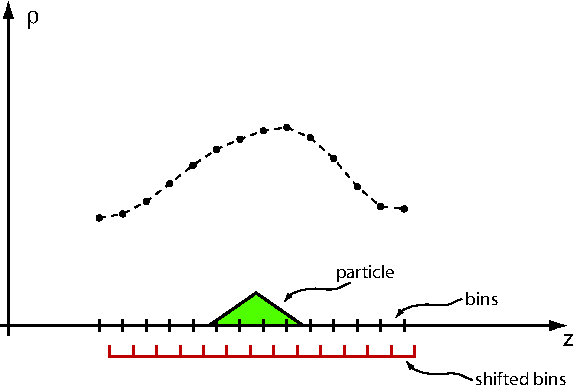
\includegraphics[height=8.4cm]{csr-bin.pdf}
\caption[CSR Calculation]
{The Coherent Synchrotron Radiation kick is calculated by dividing
longitudinally a bunch into a number of bins. To smooth the computed
densities, each particle of the bunch is considered to have a
triangular density distribution.}
\label{f:csr.bin}
\end{figure}

First a definition of some terms to avoid confusion: \vn{space charge} (SC)
and \vn{Coherent Synchrotron Radiation} (CSR) deal with the same problem
which is the direct interaction between the particles of a bunch. This is
to be differentiated from the indirect \vn{wake field} effects which are
mediated by the vacuum chamber within which a particle beam moves. The
difference between SC and CSR is that a CSR calculation takes into account
the fact that there is a delay time, due to the finite velocity of the
speed of light, so that the field felt by some particle at time $t$ due to
another (source) particle is based on the source particle's position at
some retarded time $t' \ne t$. A SC calculation, on the other hand, assumes
that the field produced by a particle at time $t$ can be can be computed
from that particle's positions at time $t$. Which type of calculation is
better depends upon what is to be simulated. Generally, the SC calculation
is preferred at lower energies where a particle's velocity is significantly
different from the speed of light.

\bmad simulates coherent synchrotron radiation (CSR) using the
formalism developed by Sagan\cite{b:csr}.  This formalism divides the
total kick received by a particle due to another particle into two
parts: One part is called the \vn{longitudinal space charge} (LSC)
kick and the other component is the \vn{coherent synchrotron
radiation} (CSR) kick. By definition, the LSC component is the
kick that would result if both particles were traveling in a straight
line. The CSR component is what is left when the LSC kick is
subtracted off from the total kick. Generally, the LSC kick is
negligible compared to the CSR kick at large enough particle energies.

Transport through a lattice element involves a beam of particles. The
lattice element is divided up into a number of slices. Transport
through a slice is a two step process.  The first step is to give all
the particles a kick due to the CSR. The second step is transport of
all particles without any interaction between particles. Note that
only the longitudinal CSR kick is implemented and transverse kicks are
ignored.

The particle-particle kick is calculated by dividing the bunch
longitudinally into a number of bins. To smooth the computed bin
densities, each particle of the bunch is considered to have a
triangular density distribution as shown in Figure~\ref{f:csr.bin}.
The particle density of a bin is calculated by summing the
contribution from all the particles. The contribution of a given
particle to a given bin is calculated from the overlap of the
particle's triangular density distribution with the bin. For the CSR
kick, the density is actually calculated for a second set of staggered
bins that have been offset by 1/2 the bin width with respect to the
first set. This gives the density at the edges of the original set of
bins. The density is considered to vary linearly between the computed
density points. For a description of the parameters that affect the
CSR calculation see Section~\sref{s:csr.params}.
 
